\section{Aufbau und Durchführung}
Der folgende Versuchsaufbau sowie die Durchführung basieren im Wesentlichen auf den Angaben in \cite{anleitungV01}.
\subsection{Aufbau}
\label{Aufbau}
Der Versuchsaufbau zur Bestimmung der Lebensdauer von Myonen ist in der \autoref{AufbauV01} abgebildet.
Er besteht aus einem Szintillatortank mit einem Volumen von ca. $50,\unit{\litre}$, an dessen beiden Enden jeweils ein Photomultiplier (PMT) angebracht ist.
Der Szintillator erzeugt Lichtblitze (Szintillationen), wenn ein Myon hindurchtritt, welche von den PMTs in elektrische Signale umgewandelt werden \cite{Teilchendetektoren}.
Diese Signale werden über Verzögerungsleitungen an Diskriminatoren mit einstellbarer Schwelle weitergeleitet. Diese unterdrücken Rauschsignale, indem sie nur Pulse oberhalb eines definierten Spannungswerts durchlassen \cite{Techniques}.
Die Pulsdauer am Ausgang dieser Diskriminatoren lässt sich ebenfalls variieren.\\
Die Ausgangssignale werden anschließend einer Koinzidenzschaltung zugeführt, 
die nur dann ein Signal erzeugt, wenn beide Pulse gleichzeitig auftreten. 
Durch diese Koinzidenzbedingung werden echte Myonensignale von zufälligen Hintergrundereignissen unterschieden.
Das daraus resultierende Signal dient als Startimpuls für die nachfolgende Zeitmessung.\\
Das Koinzidenzsignal wird sowohl über zwei AND-Gattern als auch über eine zusätzliche Verzögerungsleitung von $30\,\unit{\nano\second}$ an ein Monoflop
weitergeleitet. Dieser erzeugt ein Zeitfenster, die sogenannte Suchzeit $T_S$, innerhalb derer ein Zerfallssignal erwartet wird. 
Die beiden AND-Gatter sind mit einem Time-Amplitude-Converter (TAC) verbunden. Eines der Gatter startet die Zeitmessnung beim Eintritt
des Myons, das andere beendet sie beim Zerfall.
Über zusätzliche Leitungen, die mit einem Impulszähler verbunden sind, ist es möglich, die Anzahl der
Start- und Stoppimpulse getrennt zu erfassen. Durch diese Anordnung wird erreicht, dass die Zeitmessung startet, sobald ein Myon in das Detektor eintritt, und stoppt, wenn dieses zerfällt. 
Der TAC wandelt den Zeitabstand zwischen Start- und Stoppimpuls in eine analoge Spannung um, die proportional zur gemessenen Zeitdifferenz ist \cite{Techniques}.\\
Das Signal des TAC wird anschließend an einen Vielkanalanalysator (MCA) übergeben, der über einen PC mit entsprechender Messsoftware ausgelesen wird. Der MCA digitalisiert diese Spannungen und 
ordnet sie entsprechend ihrer Höhe diskreten Kanälen zu, wodurch ein Histogramm der Zerfallszeiten erzeugt wird \cite{Teilchendetektoren}. Zur Kalibrierung steht zudem ein Doppelimpulsgenerator zur Verfügung, 
der bei $1,\unit{\kilo\hertz}$ Doppelimpulse mit variablen Zeitabständen erzeugt.
\begin{figure}[H]
    \centering
    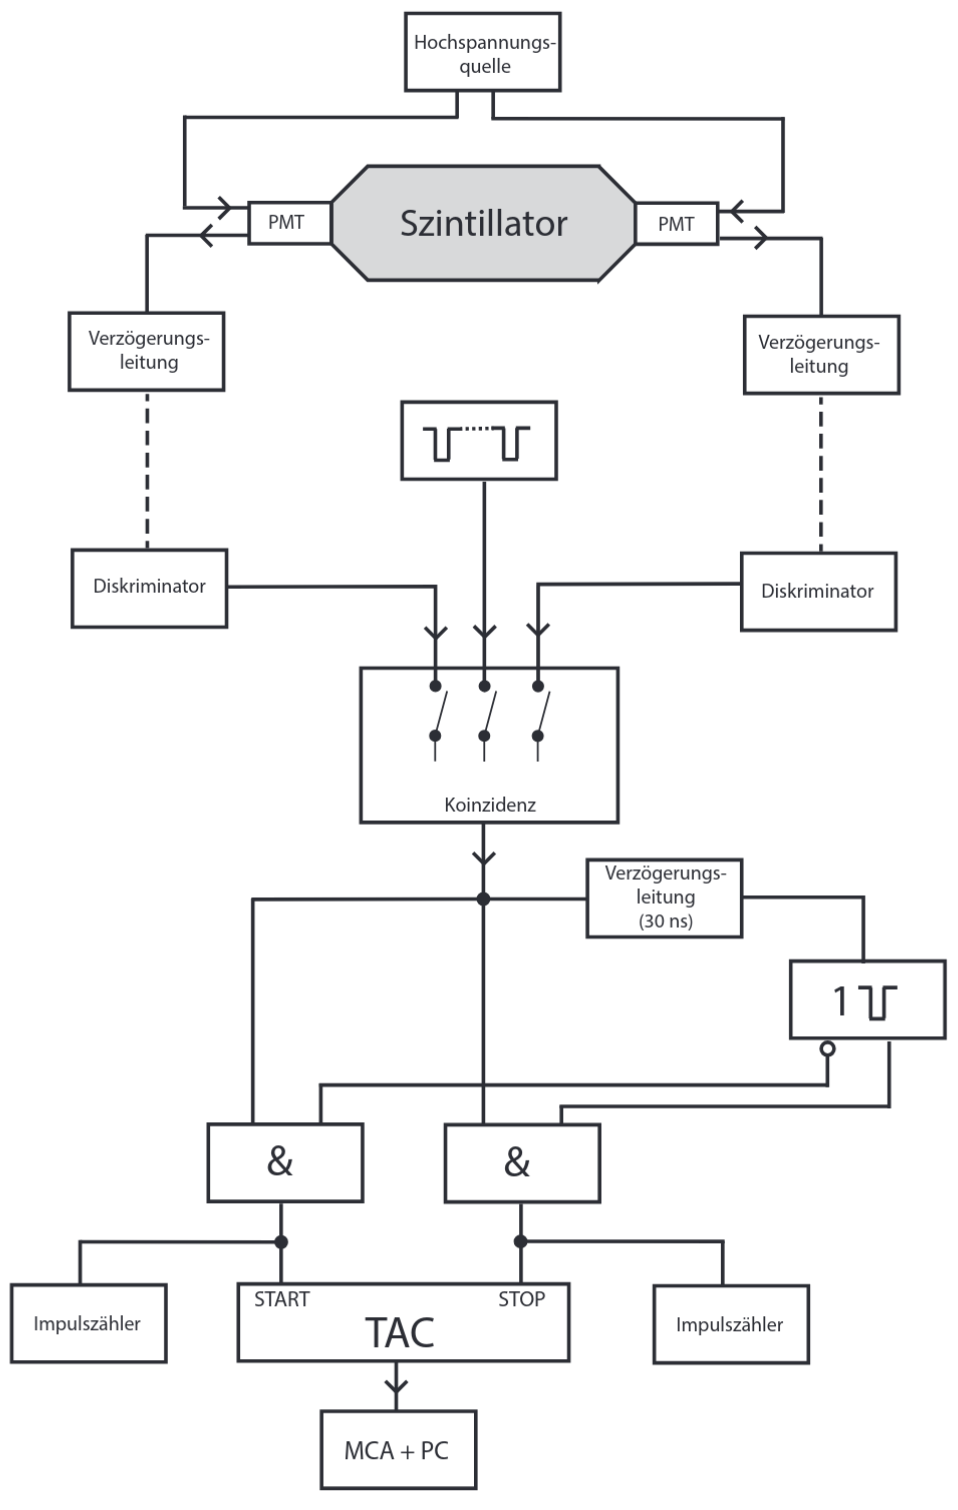
\includegraphics[width = 0.6\linewidth]{bilder/AufbauV01.png}
    \caption{Versuchsaufbau zur Bestimmung der Lebensdauer von Myonen. \cite{anleitungV01}}
    \label{AufbauV01}
\end{figure}
\subsection{Durchführung}
\label{sec:Durchführung}
Zunächst wird zur Kalibrierung des MCA ein Doppelimpulsgenerator angeschlossen. Mit diesem wird gemessen, welcher zeitliche Abstand zwischen zwei Impulsen welchem Kanal im 
MCA zugeordnet wird. Die Kalibrierung sollte mit mindestens zehn Messpunkten im Bereich von $0,3 - 9,9 \,\unit{\micro\second}$ durchgeführt werden. 
Um die Messgenauigkeit über den gesamten Bereich zu gewährleisten, sollte für alle Messpunkte die gleiche Messdauer einghalten werden. Hier wird die Messdauer von $30\,\unit{\second}$ gewählt.
Die Zählerraten können anschließend miteinander verglichen werden. Für den weitern Verlauf ist der Doppelimpulsgenerator nicht angeschlossen.\\
Sobald die Photomultiplier mit Hochspannung versorgt sind, sollten an ihren Ausgängen Spanungssingale mit unterschiedlichen Amplituden zu erkennen sein.
Dies kann mithilfe eines Oszilloskops überprüft werden.
Anschließend werden die Schwellenwerte der Diskriminatoren so eingestellt, dass an beiden Ausgängen etwa 30 Impulse pro Sekunde erzeugt werden. Dabei sollte eine
Pulsdauer von etwa $\Delta t = 10\,\unit{\nano\second}$ gewählt werden. Der Impulszähler hilft dabei, die Anzahl der Signale zu kontrollieren. Um die Koinzidenzschaltung richtig abzustimmen,
verändert man die Verzögerungsleitungen systematisch an beiden Pulse in dem Bereich $0-30\,\unit{\nano\second}$ und beobachtet die Veränderung der Impulsrate. Der gewählte Messbereich
ist dabei so groß, dass sich die Halbwertsbreite später zuverlässig bestimmen lässt. Nachdem eine geeignete Verzögerung gefunden wurde, bleibt diese für den gesamten Versuch unverändert.\\
Nach abgeschlossener Kalibrierung wird die Langzeitmessung zur Bestimmung der Lebensdauer gestartet, welche für mindestens $24\,\unit{\hour}$ durchgeführt wird.
